\chapter{Architektur}

\section{Arbeitsablauf zur Bearbeitung eines Issue}
Um eine erfolgreiche Zusammenarbeit zu gewährleisten, sind allgemein gültige Regeln nötig. Insbesondere wird festgelegt, wie die einzelnen Arbeitsschritte ablaufen sollten, um ein Issue zu bearbeiten. Zudem werden weiterhin die Zuständigkeiten geregelt.

\subsection{Verwaltung der zu bearbeitenden Issues}
Die zu bearbeitenden Issues werden auf GitHub unter Issues (\href{https://github.com/Transport-Protocol/MBC-Ping-Pong/issues}{https://github.com/Transport-Protocol/MBC-Ping-Pong/issues}) gepflegt. Um den Verlauf eines Issues darzustellen wird das Kanbanboard von GitHub (\href{https://github.com/Transport-Protocol/MBC-Ping-Pong/projects}{https://github.com/Transport-Protocol/MBC-Ping-Pong/projects}) genutzt.

\subsection{Erstellen der zu bearbeitenden Issues}
Prinzipiell kann und darf jedes Projektmitglied zu jeder Zeit Issues erstellen. Gerade bei Bugs ist dies ein gewünschtes vorgehen. In der Regel sollten dies jedoch aus Gruppensitzungen hervorgehen und durch den Architekten ausformuliert werden.\newline
Ein Issue besteht aus drei Absätzen:
\begin{itemize}
	\item \textbf{Beschreibung} \newline
	In der Beschreibung wird allgemein auf den Kontext des Issues eingegangen.
	\item \textbf{Anforderung} \newline
	In Anforderung wird die Zielvision dargestellt.
	\item \textbf{Abnahmekriterien} \newline
	In Abnahmekriterien werden alle Punkte aufgeführt, die notwendig sind, um das Issue als erfolgreich bearbeitet anzusehen.
\end{itemize}

\subsection{Das Kanbanboard}
Das Kanbanboard ist in fünf Abschnitte eingeteilt:
\begin{itemize}
	\item \textbf{Selected for Development} \newline
	Diese Spalte enthält alle Issues, die der Architekt zur Bearbeitung in nächster Zeit ausgewählt hat. Hier enthaltene Issues sind entweder durch den Architekten einem bestimmten Teammitglied zugeordnet. Diese sollten dann auch vorrangig bearbeitet werden. Oder (dies sollte der Normalfall sein) sie sind niemandem zugeordnet, dann kann sich jedes Teammitglied entscheiden, ob er das Issue bearbeitet. Gründe für das direkte zuweisen können unteranderem sein, dass es eine entsprechende vorhergehende Absprache gab, dass der Architekt das Issue speziell einem Bereich zugehörig sieht bzw. eine spezielle Paarung erreichen möchte, oder aber auch, weil ein Issue schon zu lange in "Selected for Development" verweilt. Hat sich ein Teammitglied für ein Issue entschieden, trägt er sich als Bearbeiter ein und zieht es in auf "In Development".
	\item \textbf{In Development} \newline
	In dieser Spalte verweilen alle Issues, an denen gerade entwickelt wird. Wenn die Entwicklung an einem Issue abgeschlossen ist, zieht der Bearbeiter das Issue weiter auf "Needs Review".
	\item \textbf{Needs Review} \newline
	Hier verweilen alle Issues, deren Entwicklung abgeschlossen ist, aber noch nicht geprüft wurde, ob die Abnahmebedingungen erfüllt sind. Normalerweise sollte die Abnahme durch den Architekten erfolgen. Issues, die der Architekt bearbeitet hat, muss das Review von einem anderen Teammitglied gemacht werden. Ein Issue bei dem das Review durchgeführt wird, wird in die Spalte "In Review" verschoben.
	\item \textbf{In Review} \newline
	Hier sind alle Issues enthalten, die sich gerade im Review befinden. Sind alle Abnahmekriterien erfüllt, und sind durch die Bearbeitung des Issue keine neuen Probleme/Fehler hinzugekommen, wird es in die Spalte "Done" verschoben und das Issue geschlossen. Ist dies nicht der Fall, wird ein Entsprechender Kommentar mit einer möglichst detaillierten Beschreibung des Problems an das Issue angehängt, und es wieder auf "In Development" geschoben.
	\item \textbf{Done} \newline
	Diese Spalte enthält alle abgeschlossenen Issues.
\end{itemize}

\subsection{Git}
Hier sind die Verhaltensweisen für die Nutzung von Git aufgeführt. Alles hier nicht aufgeführte kann von jedem Teammitglied nach eigenen ermessen gehandhabt werden.
\begin{itemize}
	\item \textbf{Branches} \newline
	Für jedes Issue wird ein Branch erstellt, außer es handelt sich um reine Dokumentation (im Ordner Docu). Ein Branchname folgt folgendem Muster: "\#<IssueNummer> <KurzerName>". Dadurch lässt sich
	\item \textbf{Commits} \newline
	Commits folgen folgendem Namensschema: "\#<IssueNummer> <Beschreibung>".
	\item \textbf{Push und Pull} \newline
	Es sollte möglichst häufig gepusht werden, um einen eventuellen Datenverlust zu vermeiden. Beim Pull sollte mit "--rebase" gearbeitet werden, um die Historie möglichst sauber zu halten.
	\item \textbf{Merge und Pullrequest} \newline
	Bevor ein Issue auf "Needs Review" geschoben wird, ist der Master in den Branch zu mergen und ein Pullrequest (\href{https://github.com/Transport-Protocol/MBC-Ping-Pong/pulls}{https://github.com/Transport-Protocol/MBC-Ping-Pong/pulls}) zu erstellen. Derjenige der das Issue reviewt hat, merget den Branch dann mithilfe des Pullrequests in den Master und löscht ihn.
\end{itemize}

\section{Meilensteine}
In diesem Abschnitt werden die Meilensteine festgelegt. Hierbei wird beschrieben, was wan erreicht sein sollte.
\subsection{Projekt Aufsetzen}
\begin{itemize}
	\item \textbf{Beschreibung}\newline
	Die Grundlegenden für die Entwicklung notwendigen anfangs Infrastrukturen sind aufgesetzt.
	\item \textbf{Kriterien}
	\begin{itemize}
		\item \textbf{NodeJS-Server aufsetzen} \newline
		Der NodeJS Server ist aufgesetzt und stellt eine statische Website zur Verfügung
		\item \textbf{Docker} \newline
		Eine einheitliche Umgebung wird durch Docker und Docker-Compose ermöglicht.
	\end{itemize}
	\item \textbf{Beendet:} 25.11.2016
\end{itemize}

\subsection{Prototyp (Technik)}
\begin{itemize}
	\item \textbf{Beschreibung}\newline
	Um die identifizierten technischen Risiken schnellst möglich in den Griff zu bekommen, werden diese möglichst früh bearbeitet. In dem Prototyp (Technik) soll gezeigt werden, das die kritische Technik funktioniert. Dies wird anhand von kleine losgelösten Beispielen, die aber nahe der Zielarchitektur sind gezeigt.
	\item \textbf{Kriterien}
	\begin{itemize}
		\item \textbf{Darstellung} \newline
		Es wird gezeigt, das im Webbrowser eine Flüssige Darstellung möglich ist.
		\item \textbf{Kollisionserkennung} \newline
		Es wird gezeigt, dass eine Kollisionserkennung erreichbar ist.
		\item \textbf{Kommunikation mittels WebRTC} \newline
		Architektur bedingt ist die Nutzung von WebRTC unumgänglich. Es ist zu zeigen, dass eine Verbindung von mehreren Handys zum Darstellungsmedium möglich ist.
		\item \textbf{Steuerung} \newline
		Die Steuerung soll über den Touchscreen geschehen. Es ist zu zeigen, dass es möglich ist, die Position des Fingers auf dem Touchscreen im Browser auszulesen.
		\item \textbf{Größen der Handys/Tabletts} \newline
		Unterschiedliche Handys und Tabletts haben verschiedene Größen und Formen. Somit ist ein Konzept zu erarbeiten, welches diesem Problem bei der Steuerung gerecht wird.
	\end{itemize}
	\item \textbf{Beendet:} 16.12.2016
\end{itemize}

\subsection{Release 1.0 (Zwei Spieler)}
\begin{itemize}
	\item \textbf{Beschreibung}\newline
	In diesem ersten Release ist eine Basisversion des Spieles implementiert. Es können zwei Spieler gegeneinander Spielen, indem sie ihre Schläger mit den Handys steuern. Gleichzeitig ist diese Version die minimal Version und enthält alle "Must"-Features.
	\item \textbf{Kriterien}
	\begin{itemize}
		\item \textbf{Schläger} \newline
		Für jeden Spieler existiert ein Schläger, der mit dem Handy Steuer
		\item \textbf{Ball} \newline
		Es gibt ein Ball, der sich über das Spielfeld bewegt. Kollidiert er mit einem Schläger oder der Wand, an der sich kein Schläger befindet, prallt er davon ab. Es gilt hierbei, dass der Einfallwinkel dem Ausfallwinkel entspricht. Zudem beschleunigt der Ball, wenn er mit einem Schläger kollidiert. Wenn der Ball mit der Wand hinter einem Schläger kollidiert, wir er in die Ausgangsposition versetzt und erhält die Ausgangsgeschwindigkeit.
		\item \textbf{Punkte} \newline
		Immer wenn der Ball mit der Wand hinter einem Schläger kollidiert, erhält der andere Spieler einen Punkt.
		\item \textbf{Spielende} \newline
		Das Spiel endet automatisch nach X Spielen (wobei gilt: $X \in  \mathbb{N} \land X \mod 2 = 1$ ). \textit{Das genaue X ist noch zu definieren.}
	\end{itemize}
	\item \textbf{Beendet:} 13.01.2017
\end{itemize}

\subsection{Release 1.X (Diverse Features)}
\begin{itemize}
	\item \textbf{Beschreibung}\newline
	Basierend auf der Version 1.0 wird das Spiel weiterentwickelt. Jedoch sind alle Features die hier bearbeitet werden können "Can"-Features. Daher kann es sein, dass das Release 1.X äquivalent zu dem Release 1.0 ist. Zudem sind alle hier genannten möglichen Features noch nicht näher spezifiziert und auf ihre Machbarkeit geprüft. Es gilt jedoch, dass je Umgesetztes Feature die Versionsnummer im Minorbereich um Eins steigt.
	\item \textbf{mögliche Kriterien}
	\begin{itemize}
		\item \textbf{N Spieler} \newline
		Mehr als 2 Spieler
		\item \textbf{Zusätzliche Hindernisse} \newline
		Auf dem Spielfeld sind zusätzliche Hindernisse.
		\item \textbf{Highscore-Liste} \newline
		Es wird eine Highscore-Liste geführt und angezeigt.
		\item \textbf{TBD} \newline
		To be discussed.
	\end{itemize}
	\item \textbf{Beendet:} 24.02.2017
\end{itemize}

\section{Highlevel View}
In diesem Abschnitt wird die Grob-/Gesamtarchitektur betrachtet. Hierbei wird nicht nur auf wesentliche Schnittstellen und Komponenten eingegangen. Zur engeren Auswahl standen zwei mögliche Ansätze. Es werden beide betrachtet, und erläutert warum der Ansatz 2 umgesetzt werden wird.
\subsection{Ansatz 1}
Der Ansatz 1 verfolgt den Klassischen Client-Server-Ansatz. Hierbei dient der Server als zentrale Instanz, die alle signifikanten Logikoperationen übernimmt. Die Clients dienen lediglich zur Ein-/Ausgabe.
\begin{figure}[ht]
	\centering
	\includegraphics[width=0.9\textwidth]{architecture/highLevelAnsatz1.png}
	\caption{Highlevel Ansatz 1}
	\label{fig1}
\end{figure}
\subsubsection{Server}
Der Server stellt die statischen Inhalte (HTML, CSS, JS) bereit. Zudem enthält er die gesamte Spiellogik. Der Server empfängt Steuerinformationen vom ControlClient, verarbeitet diese und sendet einen aktuellen Gamestate an den OutputClient.
\subsubsection{ControlClient}
Der ControlClient erfasst die Steuereingaben des Nutzers und sendet sie an den Server.
\subsubsection{OutputClient}
Der OutputClient empfängt den Gamestate vom Server und aktualisiert die Anzeige entsprechend.
\subsubsection{Analyse}
Einerseits ist dieser Ansatz architektonisch sehr einfach umzusetzen, da es eine zentrale Instanz gibt und Seperation of Concerns Architektur bedingt unterstützt wird. Zudem ist es möglich ein Spiel auf mehreren OutputClients darzustellen. Da sich die Clients mit dem Server verbinden, ist der Einsatz von WebSockets möglich. Mit socket.io gibt es eine sehr gute Abstraktionsschicht für WebSockets. Andererseits kann durch den Einsatz von WebSockets ein nicht zu vernachlässigendes Delay entstehen, da diese auf TCP basieren. Um diesem zu begegnen ist der Einsatz des WebRTC Protokollstacks notwendig. Zudem muss der Server die Zuordnung der ControlClients und OutputClients zu einem Spiel organisieren. Außerdem sind zwei Netzwerkübertragungen von Nöten, damit die Eingabe des Spielers auf dem OutputClient sichtbar wir. Dadurch wird das Netzwerk doppelt belastet, und es ist zweimal das Übertragungsdelay vorhanden.
\subsection{Ansatz 2}
\begin{figure}[ht]
	\centering
	\includegraphics[width=0.9\textwidth]{architecture/highLevelAnsatz2.png}
	\caption{Highlevel Ansatz 2}
	\label{fig2}
\end{figure}
\subsubsection{Server}
Der Server stellt die statischen Inhalte (HTML, CSS, JS) bereit. Zudem fungiert er als zentrale Instanz für den WebRTC-Protokollstack
\subsubsection{ExternerServer}
Der externe Server ist ein öffentlicher Stun-/Turn-/Ice-Server, der beispielsweise von Google bereitgestellt wird.
\subsubsection{ControlPeer}
Der ControlPeer erfasst die Steuereingaben des Nutzers und sendet sie an den DisplayPeer.
\subsubsection{DisplayPeer}
Der DisplayPeer ist ein Fat-Client. Er enthält die gesamte Spiellogik und empfängt über den WebRTC-Protokollstack direkt die Steuereingaben des Spielers. Zudem zeigt er das Spiel an.
\subsubsection{Analyse}
Der Ansatz 2 ist architektonisch recht Komplex, da die Aufteilung auf Client und Server wegfällt, und somit die native Unterstützung von Seperation of Concern nicht gegeben ist. Es muss während der Entwicklung verstärkt darauf geachtet werden, das die Trennung von Spiellogik und Ausgabe eingehalten wird. Zu dem ist man auf den WebRTC-Protokollstack angewiesen, da die Peers direkt miteinander Kommunizieren müssen. Außerdem ist man auf einen einzelnen DisplayPeer beschränkt. Andererseits erfolgt die Übertragung der Steuerung direkt von dem ControlPeer an den DisplayPeer, dadurch ist das kleinst mögliche Delay zwischen Eingabe, Verarbeitung und Ausgabe gewährleistet. Außerdem ermöglicht der Einsatz von WebRTC den Einsatz von UDP als Transportprotokoll, wodurch das Delay weiter verringer werden kann, da UDP Verbindungslos ist.
\subsection{Fazit}
Auch wenn der Ansatz 2 zunächst komplexer erscheint und einen geringeren Funktionsumfang bietet, da nur ein AusgabeClient pro Spiel unterstützt wird und WebRTC eingesetzt werden muss, überwiegen doch die Vorteile dieses Ansatzes. Durch die fehlende zweite Netzwerkübertragung und der mögliche Einsatz von UDP, werden Delays minimiert. Gleichzeitig wird mehr Rechenleistung auf die Clients ausgelagert und eine aufwändige Verwaltung, welcher Spieler zu welchem Spiel gehört ist auch nicht notwendig.

\section{Risiken}
In diesem Kapitel wird auf die Risiken eingegangen, die zu Schwierigkeiten bei der Projektdurchführung führen können. Die Auswirkungen und Eintrittswahrscheinlichkeit werden in 3 Kategorien eingeteilt: "1:Gering, 2:Mittel, 3: Hoch". Das potenzielle Risiko ist das Produkt aus Auswirkungen und Eintrittswahrscheinlichkeit.
\subsection{Technische Risiken}
Zunächst wird auf die technischen Risiken eingegangen
\subsubsection{Darstellung ist nicht möglich}
\begin{itemize}
	\item \textbf{Beschreibung:} \newline
	Gerade bei Ping-Pong wird die Bewegung des Balls irgendwann sehr schnell. Dies muss trotzdem im Browser darstellbar sein, ohne das es ruckelt.
	\item \textbf{Eintrittsgründe;}
	\begin{itemize}
		\item Das gewählte Grafikframework ist nicht leistungsfähig genug.
		\item Das gewählte Grafikframework wurde nicht richtig genutzt.
		\item Das Zielsystem ist nicht Leistungsfähig genug.
	\end{itemize}
	\item \textbf{Folgen:}
	\begin{itemize}
		\item Das Spielen ist nicht möglich => Projektfehlschlag.
	\end{itemize}
	\item \textbf{Eintrittswahrscheinlichkeit:} 2
	\item \textbf{Auswirkungen:} 3
	\item \textbf{Risiko:} 6
	\item \textbf{Maßnahmen:}
	\begin{itemize}
		\item Bereits im Prototyp eine Beispielimplementierung durchführen.
		\item Möglichst früh einen Test auf der Zielplattform absolvieren.
	\end{itemize}
\end{itemize}
\subsubsection{Kollisionserkennung funktioniert nicht}
\begin{itemize}
	\item \textbf{Beschreibung:} \newline
	Durch die schnelle Ballbewegung bei Ping-Pong ist eine gute Kollisionserkennung notwendig.
	\item \textbf{Eintrittsgründe;}
	\begin{itemize}
		\item Die gewählte Physicsengine ist nicht leistungsfähig genug.
		\item Die gewählte Physicsengine wurde nicht richtig genutzt.
		\item Das Zielsystem ist nicht Leistungsfähig genug.
	\end{itemize}
	\item \textbf{Folgen:}
	\begin{itemize}
		\item Das Spielen ist nicht möglich => Projektfehlschlag.
	\end{itemize}
	\item \textbf{Eintrittswahrscheinlichkeit:} 2
	\item \textbf{Auswirkungen:} 3
	\item \textbf{Risiko:} 6
	\item \textbf{Maßnahmen:}
	\begin{itemize}
		\item Bereits im Prototyp eine Beispielimplementierung durchführen.
		\item Möglichst früh einen Test auf der Zielplattform absolvieren.
	\end{itemize}
\end{itemize}
\subsubsection{Kommunikation mittels WebRTC funktioniert nicht}
\begin{itemize}
	\item \textbf{Beschreibung:} \newline
	Um die Übertragung in akzeptabler Geschwindigkeit zu gewährleisten, ist der Einsatz von WebRTC unausweichlich. WebRTC ist jedoch absolutes Neuland für das gesamte Team.
	\item \textbf{Eintrittsgründe;}
	\begin{itemize}
		\item WebRTC wird nicht korrekt genutzt.
		\item Im Zielnetzwerk wird die Verwendung durch Firewalls behindert.
	\end{itemize}
	\item \textbf{Folgen:}
	\begin{itemize}
		\item Die Architektur muss von Fat-Client Ansatz auf einen Serverzentrierten Ansatz umgestellt werden => Projektverzögerung.
	\end{itemize}
	\item \textbf{Eintrittswahrscheinlichkeit:} 2
	\item \textbf{Auswirkungen:} 2
	\item \textbf{Risiko:} 4
	\item \textbf{Maßnahmen:}
	\begin{itemize}
		\item Bereits im Prototyp eine Beispielimplementierung durchführen.
		\item Möglichst früh einen Test auf der Zielplattform absolvieren.
	\end{itemize}
\end{itemize}
\subsubsection{Steuerung ist nicht möglich}
\begin{itemize}
	\item \textbf{Beschreibung:} \newline
	Das auslesen der Position des Fingers auf dem Bildschirm über den Browser funktioniert nicht, bzw. nicht schnell genug.
	\item \textbf{Eintrittsgründe;}
	\begin{itemize}
		\item Zu altes Handy verwendet (Browser unterstützt es nicht).
		\item Schnittstelle nicht korrekt verwendet
	\end{itemize}
	\item \textbf{Folgen:}
	\begin{itemize}
		\item Das Spiel ist nicht Steuerbar => Projektfehlschlag.
	\end{itemize}
	\item \textbf{Eintrittswahrscheinlichkeit:} 1
	\item \textbf{Auswirkungen:} 3
	\item \textbf{Risiko:} 3
	\item \textbf{Maßnahmen:}
	\begin{itemize}
		\item Bereits im Prototyp eine Beispielimplementierung durchführen.
	\end{itemize}
\end{itemize}
\subsection{Konzeptuelle Risiken}
\subsubsection{Steuerung ist nicht Fair}
\begin{itemize}
	\item \textbf{Beschreibung:} \newline
	Gerade mit dem Prinzip des Browser basierten Ansatzes werden sehr viele unterschiedliche Endgerätetypen angesprochen. Jedes Endgerät hat jedoch eine andere Bildschirmgröße und Pixeldichte.
	\item \textbf{Eintrittsgründe;}
	\begin{itemize}
		\item Es möchten Personen mit unterschiedlichen Endgeräten gegeneinander antreten
	\end{itemize}
	\item \textbf{Folgen:}
	\begin{itemize}
		\item Das Spiel ist unfair => geringere Akzeptanz.
	\end{itemize}
	\item \textbf{Eintrittswahrscheinlichkeit:} 3
	\item \textbf{Auswirkungen:} 1
	\item \textbf{Risiko:} 3
	\item \textbf{Maßnahmen:}
	\begin{itemize}
		\item Das Risiko wird durch die weitergehende Analyse, und dem Entwurf eines möglichst Fairen Steuerungskonzeptes verringert.
		\item Ggf. zum Teil ignorieren
	\end{itemize}
\end{itemize}
\subsection{Organisatorische Risiken}
\subsubsection{Temporärer Personalausfall}
\begin{itemize}
	\item \textbf{Beschreibung:} \newline
	Es kann jederzeit zu einem temporären Personalausfall kommen.
	\item \textbf{Eintrittsgründe;}
	\begin{itemize}
		\item Krankheit.
		\item Klausuren.
		\item Unmotiviertheit.
	\end{itemize}
	\item \textbf{Folgen:}
	\begin{itemize}
		\item Arbeitskraftmangel => Projektverzögerung.
		\item Fachwissensmangel => Projektverzögerung.
	\end{itemize}
	\item \textbf{Eintrittswahrscheinlichkeit:} 3
	\item \textbf{Auswirkungen:} 1
	\item \textbf{Risiko:} 3
	\item \textbf{Maßnahmen:}
	\begin{itemize}
		\item Puffer einplanen.
		\item Möglichst wenig Must-Anforderungen definieren.
	\end{itemize}
\end{itemize}
\subsubsection{Kompletter Personalausfall}
\begin{itemize}
	\item \textbf{Beschreibung:} \newline
	Es kann jederzeit zu einem temporären Personalausfall kommen.
	\item \textbf{Eintrittsgründe;}
	\begin{itemize}
		\item Krankheit.
		\item Unmotiviertheit.
	\end{itemize}
	\item \textbf{Folgen:}
	\begin{itemize}
		\item Arbeitskraftverlust => Projektverzögerung.
		\item Fachwissensverlust => Projektverzögerung.
	\end{itemize}
	\item \textbf{Eintrittswahrscheinlichkeit:} 2
	\item \textbf{Auswirkungen:} 2
	\item \textbf{Risiko:} 4
	\item \textbf{Maßnahmen:}
	\begin{itemize}
		\item Puffer einplanen.
		\item Möglichst wenig Must-Anforderungen definieren.
	\end{itemize}
\end{itemize}

\section{Reviews}
\subsection{\href{https://github.com/Transport-Protocol/MBC-Ping-Pong/issues/3}{Auswahl einer geeigneten 2D-/Physiksengine}}
\begin{itemize}
	\item \textbf{Datum:} 05.12.16
	\item \textbf{Prüfung der Anforderungen:}
	\begin{itemize}
		\item \checkmark Aufruf der Seite http://<IpDesNodeJsServers>:<HttpPortDesNodeJsServers>/test2DEngine.html zeigt die Testseite.
		\item \checkmark Ein quadratischer Bereich mit einer Form in der Mitte auf dem Bildschirm wird dargestellt.
		\item \checkmark In diesem Bereich bewegt sich eine Form (am besten eine Kugel) waagerecht von Links nach Rechts.
		\item \checkmark Kollidiert die Form mit der rechten Wand, bewegt sich die Form von Rechts nach Links.
		\item \checkmark Kollidiert die Form mit der linken Wand, bewegt sich die Form von Links nach Rechts.
	\end{itemize}
	\item \textbf{Prüfung des Codes:}
	\begin{itemize}
		\item Der Code ist strukturiert und lesbar.
		\item Bis auf 2 Zeilen ist der Code verständlich:
		\begin{itemize}
			\item this.ball.body.immovable = true; \newline
			Ein besserer Kommentar, warum wäre gut gewesen. Nach einigem suchen, gehe ich davon aus, dass nur Objekte, die mit dem Ball kollidieren, beeinflusst werden, aber nicht der Ball selbst.\newline
			Dieses Verhalten ist zunächst OK, sollte jedoch bei späteren Features noch einmal geprüft werden.
			\item this.ball.body.bounce.set(1); \newline
			Es funktioniert in der momentan verwendeten Version, daher ist es OK, sollte jedoch geprüft werden. Laut Dokumentation (\href{http://phaser.io/docs/2.6.2/Phaser.Physics.Ninja.Body.html\#bounce}{http://phaser.io/docs/2.6.2/Phaser.Physics.Ninja.Body.html\#bounce}) Sollte der Wert zwischen 0 und 1 liegen, also nicht 1.0 sein. Empfohlen wird ein wert von 0.999. Eine Prüfung ergab, das auch Werte oberhalb von 1.0 akzeptiert werden. Dies führt dann zu einer Beschleunigung des Balls.
		\end{itemize}
	\end{itemize}
\end{itemize}

\FloatBarrier

\section{Prototyp}
In diesem Kapitel wird der Prototyp behandelt.

\subsection{Schnittstellen}
Dieses Diagramm (Abbildung \ref{Prototyp Schnittstellen - Klassendiagram}) dient dem gemeinsamen Verständnis, welche Klasse welche Schnittstelle bietet.
\begin{figure}[ht]
	\centering
	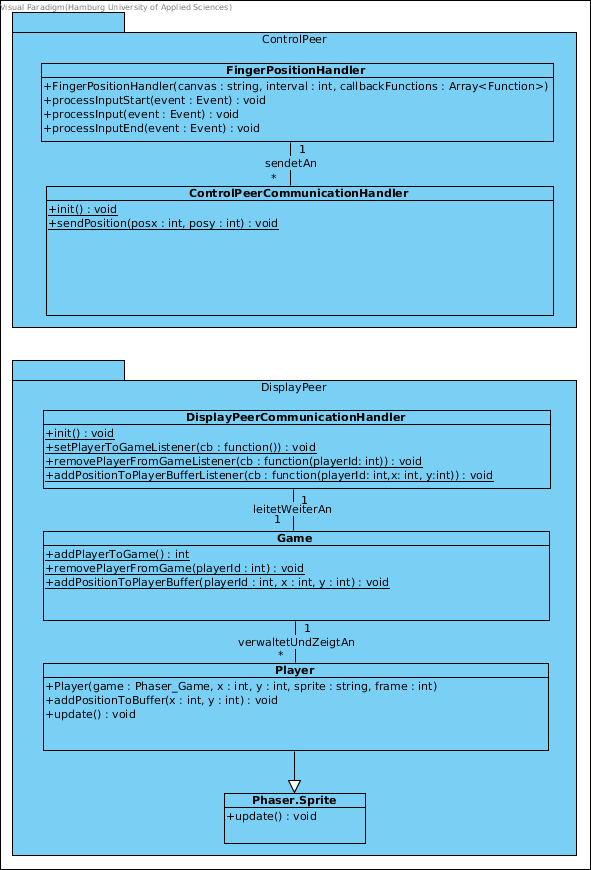
\includegraphics[width=0.9\textwidth]{architecture/PrototypeClassDiagram.png}
	\caption{Prototyp Schnittstellen - Klassendiagram}
	\label{Prototyp Schnittstellen - Klassendiagram}
\end{figure}

\subsection{Fachlicher Ablauf}
Im fachlichen Ablauf (Abbildung \ref{Prototyp fachlicher Ablauf - Sequenzdiagramm}) wird dargestellt, wie sich das Programm verhalten soll. Es wird jedoch nicht auf genaue Implementierungsdetails wert gelegt. Er dient dem allgemeine Verständnis, wie der Programmablauf sein soll. Auch die Funktionsnamen bei fremd-APIs dienen lediglich der Beschreibung, welches Verhalten von der API erwartet wird. \textbf{Allerdings sollte der Ablauf später im Programmcode ersichtlich sein.}
\begin{figure}[ht]
	\centering
	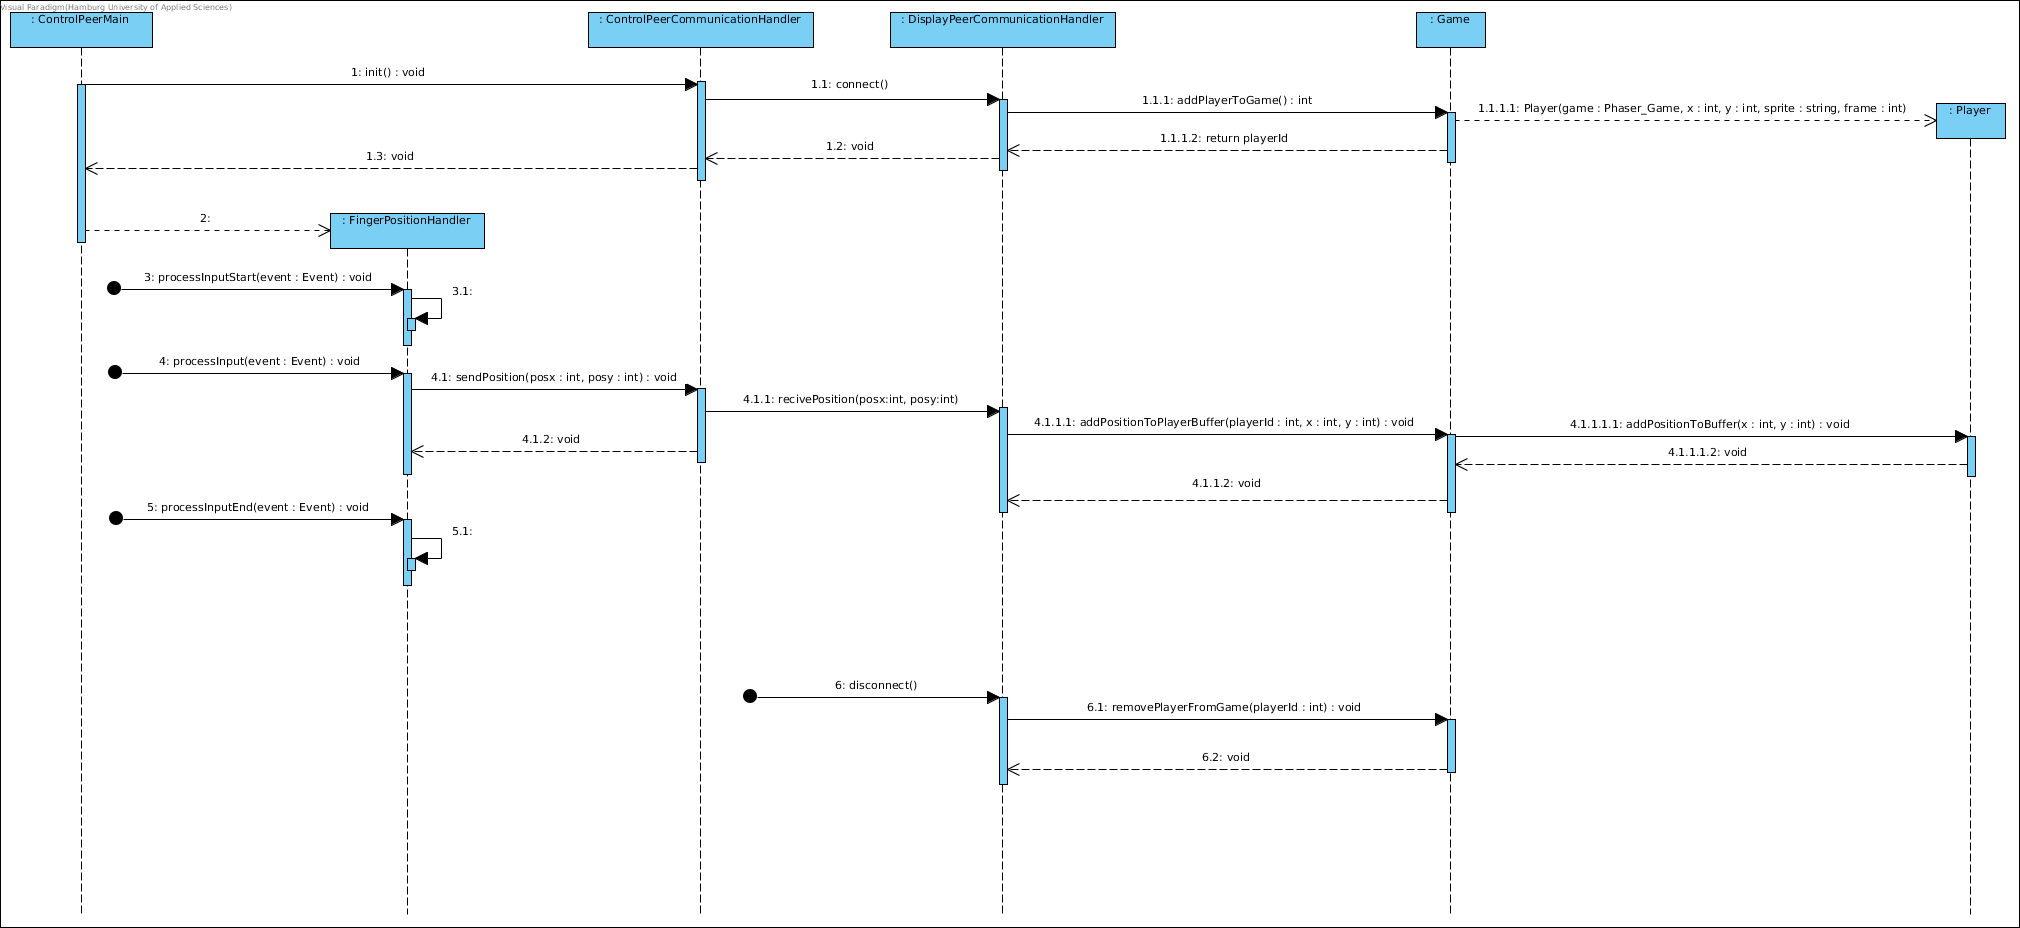
\includegraphics[width = 0.9\textheight, angle=270]{architecture/PrototypeSequenceDiagram.png}
	\caption{Prototyp fachlicher Ablauf - Sequenzdiagramm}
	\label{Prototyp fachlicher Ablauf - Sequenzdiagramm}
\end{figure}

\FloatBarrier

\section{Release 1.0}
	\subsection{MookUps} \label{mookups}
		Die Mookups (\ref{Mookup - Initial} - \ref{Mookup - GameEnded}) zeigen die Zustände des Spiels und die einzelnen Komponenten (in den MookUps durch grüne Namen gekennzeichnet) werden beschrieben. Im Abschnitt \ref{states} wird gezeigt, wie die einzelnen States in einander Überführt werden.
		\subsubsection{Beschreibung der Komponenten}
		\begin{itemize}
			\item \textbf{Spieler 1:} Spieler, der den Schläger auf der linken Spielfeldseite steuert.
			\item \textbf{Spieler 2:} Spieler, der den Schläger auf der rechten Spielfeldseite steuert.
			\item \textbf{Spielfeld:} Bereich, in dem das Spiel durch Phaser dargestellt wird.
			\item \textbf{Wand 1:} Wand hinter dem Schläger 1. Wird diese getroffen, erhält Spieler 2 einen Punkt.
			\item \textbf{Wand 2:} Wand hinter dem Schläger 2. Wird diese getroffen, erhält Spieler 1 einen Punkt.
			\item \textbf{Wand 3:} Seitenwände, die lediglich zur Spielfeldbegrenzung dienen.
			\item \textbf{Schläger 1:} Schläger der durch Spieler 1 gesteuert wird. Er kann sofort nach der Erstellung durch Spieler 1 bewegt werden.
			\item \textbf{Schläger 2:} Schläger der durch Spieler 2 gesteuert wird. Er kann sofort nach der Erstellung durch Spieler 2 bewegt werden.
			\item \textbf{Ball:} Der Ball bewegt sich über das Spielfeld, und muss mit den Schlägern davon abgehalten werden, die Wand hinter den Schlägern zu treffen. Trifft der Ball Wand 1 oder 2, wird er in die Ausgangsposition gesetzt und erhällt seine Ausgangsgeschwindigkeit, sowie eine zufällig Richtung. Trifft er Wand 3 oder einen Schläger, prallt er von diesem ab und wird beschleunigt.
			\item \textbf{Punkte:} Anzeige des aktuellen Spielstandes, im Format <Treffer auf Wand2> : <Treffer auf Wand 1>.
			\item \textbf{JoinGamePanel:} Hier werden alle Informationen angezeigt, die benötigt werden, um einem Spiel beizutreten.
			\begin{itemize}
				\item \textbf{QR-Code:} URL 1 als QR-Code
				\item \textbf{URL 1:} URL, um dem Spiel beizutreten.
			\end{itemize}
			\item \textbf{Timer:} Restzeit bis zum Eintreten eines Events.
		\end{itemize}
		\begin{figure}[!htb]
			\centering
			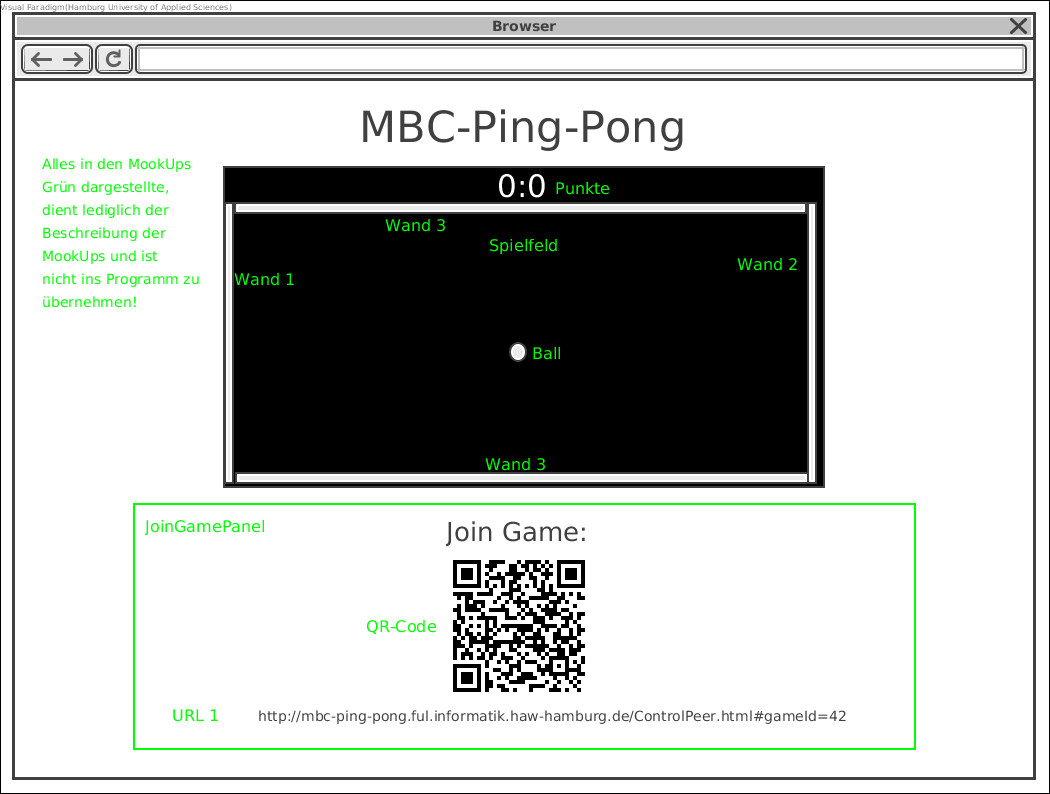
\includegraphics[width=0.65\textwidth]{architecture/Mookup - Initial.png}
			\caption{Mookup - Initial}
			\label{Mookup - Initial}
		\end{figure}
		
		\begin{figure}[!htb]
			\centering
			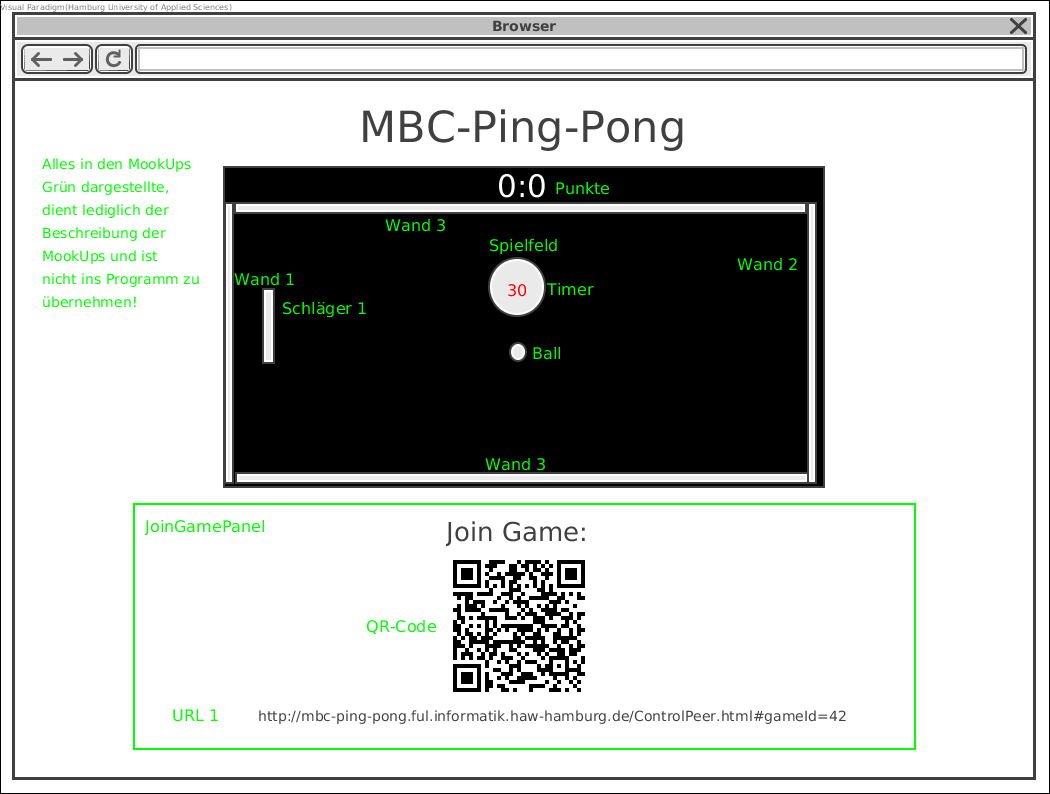
\includegraphics[width=0.65\textwidth]{architecture/Mookup - FirstPlayerConnected.png}
			\caption{Mookup - FirstPlayerConnected}
			\label{Mookup - FirstPlayerConnected}
		\end{figure}
		
		\begin{figure}[!htb]
			\centering
			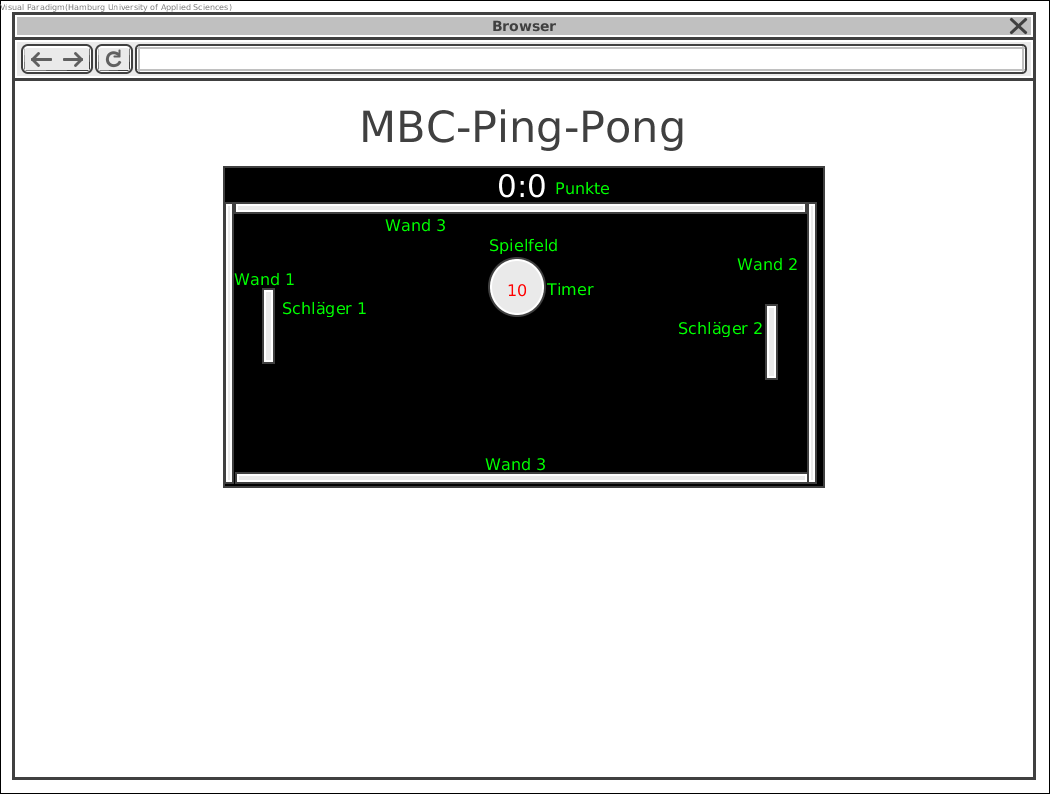
\includegraphics[width=0.65\textwidth]{architecture/Mookup - SecondPlayerConnected.png}
			\caption{Mookup - SecondPlayerConnected}
			\label{Mookup - SecondPlayerConnected}
		\end{figure}
		
		\begin{figure}[!htb]
			\centering
			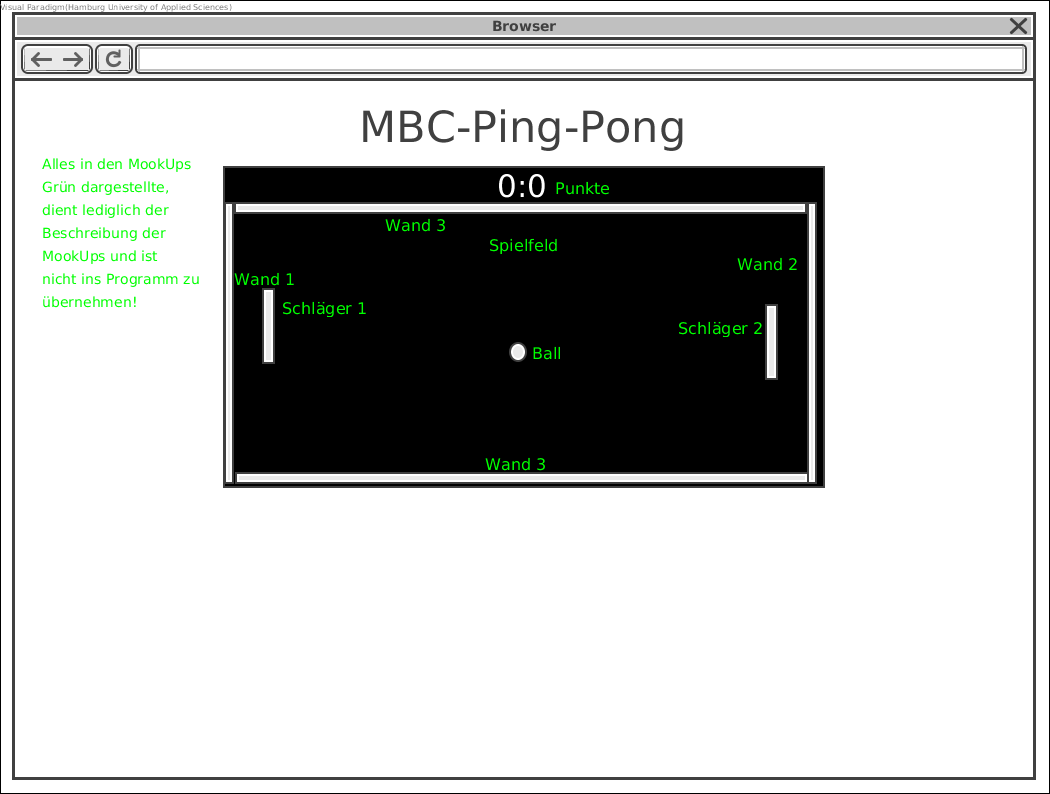
\includegraphics[width=0.65\textwidth]{architecture/Mookup - GameRunning.png}
			\caption{Mookup - GameRunning}
			\label{Mookup - GameRunning}
		\end{figure}
		
		\begin{figure}[!htb]
			\centering
			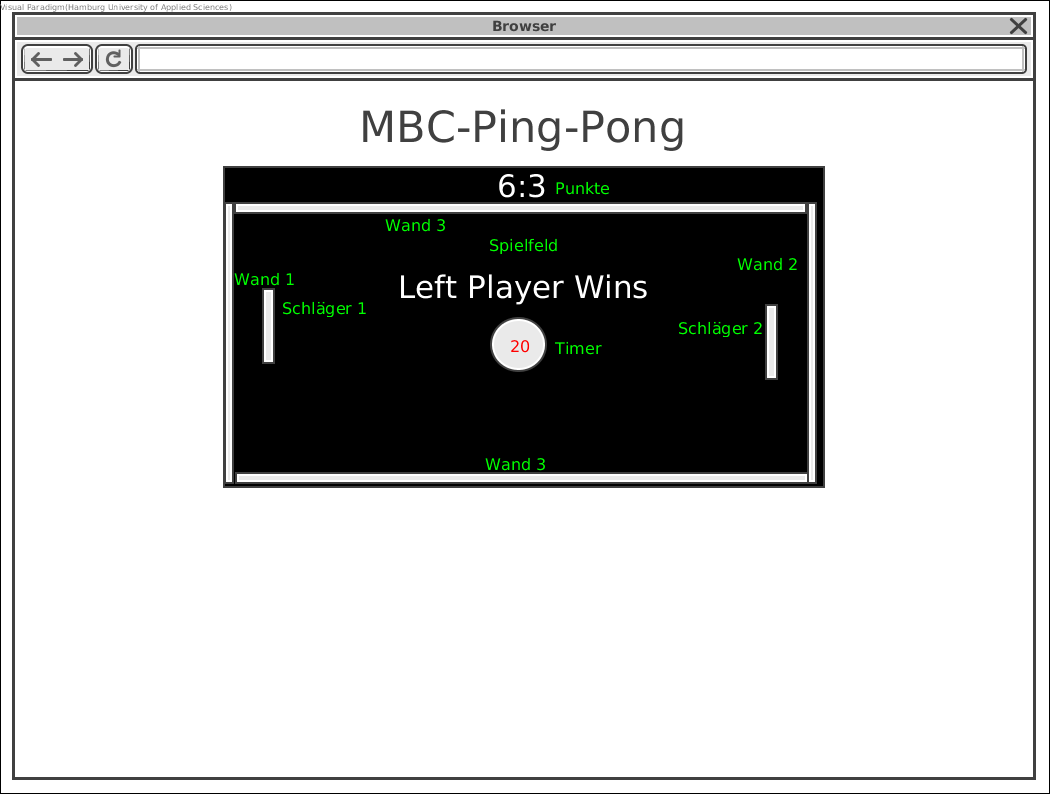
\includegraphics[width=0.65\textwidth]{architecture/Mookup - GameEnded.png}
			\caption{Mookup - GameEnded}
			\label{Mookup - GameEnded}
		\end{figure}

	\FloatBarrier
	\subsection{States} \label{states}
		Hier wird gezeigt, wie die States ineinander über gehen. Zu den grünen Zuständen gibt es Mookups in \ref{mookups}.
		\begin{figure}[!htb]
			\centering
			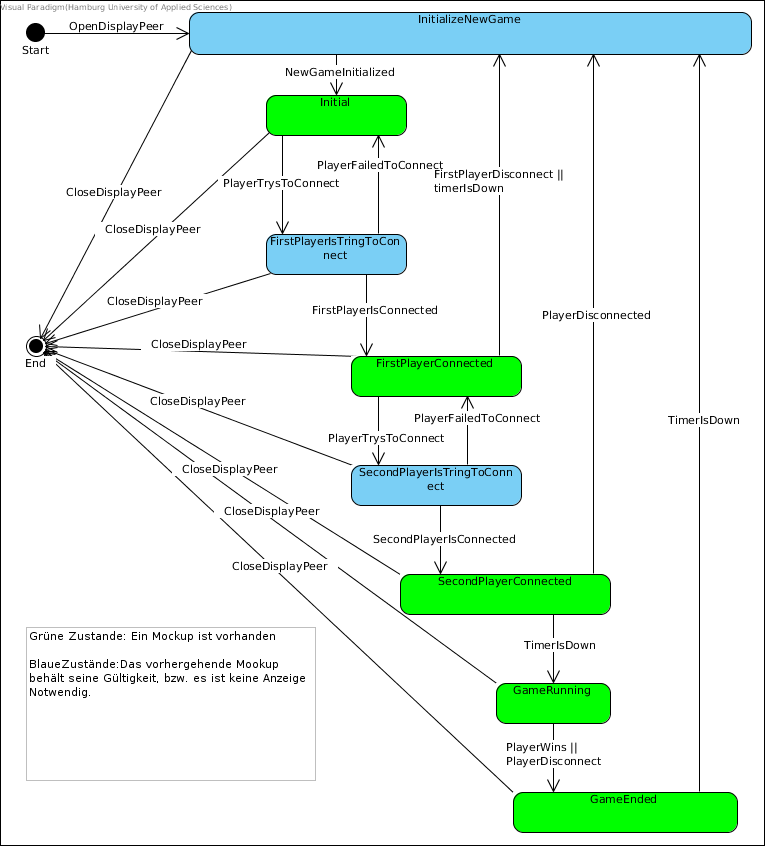
\includegraphics[width=0.9\textwidth]{architecture/StateMachineRelease1.0.png}
			\caption{Statemachine Release 1.0}
			\label{Statemachine Release 1.0}
		\end{figure}
	\FloatBarrier	
	\subsection{Klassendiagramm} \label{states}
		\begin{figure}[!htb]
			\centering
			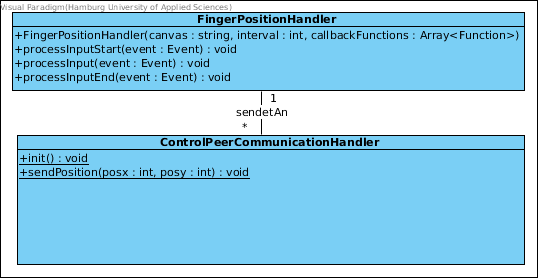
\includegraphics[width=0.9\textwidth]{architecture/Release1.0ClassDiagramControlPeer.png}
			\caption{ControlPeer ClassDiagram Release 1.0}
			\label{ControlPeer ClassDiagram Release 1.0}
		\end{figure}
		\begin{figure}[!htb]
			\centering
			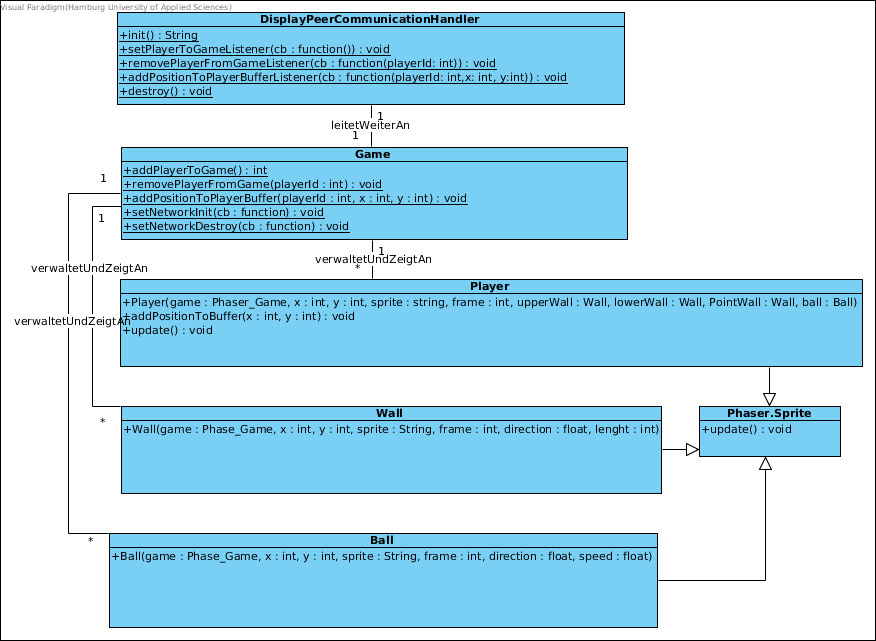
\includegraphics[width=0.9\textwidth]{architecture/Release1.0ClassDiagramDisplayPeer.png}
			\caption{DisplayPeer ClassDiagram Release 1.0}
			\label{DisplayPeer ClassDiagram Release 1.0}
		\end{figure}
